\chapter{Experimentaci\'on y Resultados}\label{chapter:experiments}
En este cap\'itulo se evaluan los resultados obtenidos por AutoGOAL multiobjetivo tras aplicarse sobre tres corpus de datos aplicando precis\'on contra recobrady y \textit{f-score} contra tiempo de entrenamiento y precisi\'on contra recobrado.

Precisi\'on es una m\'etrica que mide las muestras clasificadas correctamente entre todas las muestras extra\'idas. Recobrado mide las muestras clasificadas correctamente sobre todas las extra\'idas.
\textit{F-score} es el promedio harm\'onico entre precisi\'on y recobrado.
Tiempo de entrenamiento es un estimado que mide cuanto toma dado una soluci\'on en realizar el proceso de entrenamiento.

Se utiliza el par de metricas precisi\'on y recobrado que son m\'etricas que pueden tener comportamientos variados. Existen conjuntos de entrenamiento donde es posble maximizar ambas y existen otros donde es obligatorio realizar trade-offs y no es posible maximizar ninguna.

Se utilza \textit{f-score} contra tiempo de entrenamiento para probar si es posible dirigir efectivamente  la b\'usqueda maximizando la relevancia y minimizando el tiempo de ejecuci\'on. Es posible utilzar tambi\'en precisi\'on, recobrado junto con tiempo de entrenamiento pero con el objetivo de mantener la representaci\'on m\'as visible se utiliza f-score

\section{Corpus de Evaluaci\'on}
Se utilizan tres corpus de datos para comprobar el comportamiento del sistema cuando optmiza para varias m\'etricas simult\'aneamente. Los corpus se escogen de distintos tamaños y cada uno representa versiones distintas del problema de aprendizaje supervisado.

\subsection{CARS}
Cars es un corpues que representa un conjutno de carros con ciertas caracter\'isticas cat\'alogadas cualitativamente (ver \ref{implementation:table:cars:attributes}). El objetivo con este corpus es aprender a clasificar los carros de  acuerdo a sus atributos  en inaceptable, aceptable, bueno o muy bueno (\ref{implementation:table:cars:classes}). El dataset no tiene valores desconocidos.

\begin{table}[ht]
    \centering
    \parbox{.45\linewidth}{
    \begin{tabular} { |l|c| }
        \hline
        Atributos & Valores \\
        \hline
        \hline
        buying & v-high, hihg, med, low \\
        \hline
        maintance &  v-high, hihg, med, low\\
        \hline
        doors & 2, 3, 4, 5-more\\
        \hline
        persons & 2, 4, more\\
        \hline
        lug\_boot & small, med, big\\
        \hline
        safety & low, med, high\\
        \hline
    \end{tabular}
    \caption{Tipos de Atributos en Cars}
    \label{implementation:table:cars:attributes}
    }
    \qquad
    \parbox[t]{.45\linewidth}{
    \begin{tabular} {|l|c|c|}
        \hline
        Clases & N & \% \\
        \hline
        \hline
        unacc & 1210 & 70.023\%\\
        \hline
        acc & 384 & 22.222\%\\
        \hline
        good & 69 & 3.993\%\\
        \hline
        v-good & 65 & 3.762\%\\
        \hline
    \end{tabular}
    \caption{Distribuci\'on de clases en Cars}
    \label{implementation:table:cars:classes}
    }
\end{table}

\subsection{HAHA}
Humor Analysis based on Human Annotation (HAHA), un conjunto de datos que contiene \textit{tweets} en espa\~nol en texto plano codificado en utf-8. Se quiere construir un clasificador que pueda catalogarlos correctamente entre si son humor\'isticos o no. Contiene un total de 30000 tweets donde se utilizan 24000 para entrenaiento y 6000 para evaluaci\'on.

\begin{table}[ht]
    \centering
    \begin{tabular} {|l||c|c|c|}
        \hline
        & Entrenamiento & Evaluaci\'on & Total \\
        \hline
        \hline
        Tweets & 24000 & 6000 & $30000$\\
        \hline
        Graciosos & 9253 & 2342 & 11595\\
        \hline
        No graciosos & 14 757 & 3 658 & 18 405\\
        \hline
        Puntuaci\'on Promedio & 1305 & 275 & 1580\\
        \hline
    \end{tabular}
    \caption{Distribuci\'on de clases en HAHA}
    \label{implementation:table:haha}
\end{table}

\subsection{MEDDOCAN}

Una colecci\'on de 1000 casos cl\'inicos y sus anotaciones PHI; cada uno conformado con aproximadamente de 33 oraciones o 495 palabras. Cada caso cl\'inico est\'a codificado en texto plano en UTF8 y las anotaciones est\'an en formato BRAT. El objetivo es predecir dichas anotaciones.

\paragraph{Hardware} Los experimentos fueron ejecutados en un equipo con las siguientes propiedades: CPU AMD R5 3550h y 32 GB de RAM.

\section{Resultados y An\'alisis}

A continuaci\'on se muestran los resultados y anal\'isi de aplicar AutoGOAL Multiobjetivo a los distintos corpus. En las gr\'aficas solo se tiene en cuenta la puntuaci\'on de relevancia respecto a los datos entrenamiento y no a los datos de prueba. Los puntos  grises marcan las mejores soluciones encontradas en cada generaci\'on.  La tonalidad de los puntos var\'ia de acuerdo en que iteraci\'on del algoritmo fue encontrado; a medida que avanzan las generaciones esos aparecen m\'as oscuros. Los puntos marcados con cruces rojas representan las mejores soluciones encontradas por el algoritmo y conforman una aproximaci\'on del frente de Pareto.

Para cada conjunto de datos se utilizaron param\'etros distintos debido fundamentalmene a que cada corpus representa problemas con diferente complejidad y cantidad de datos.

\subsection{Cars}
La aplicaci\'on de AutoGOAL en cars  utilza una poblaci\'on total de 40 individuos por generaci\'on, 1 hora de tiempo m\'aximo y 10 segundos de tiempo l\'imite por \textit{pipeline}. Se utilizaron las implementaciones de \textit{f-score}, \textit{precision} y \textit{recall} de scikit-learn con el promedio \textit{weighted} utilizado para problemas de clasificaci\'on multiclase que pueden tener un desbalance en las clases existentes.

\subsubsection{F-Score contra Tiempo de Entrenamiento}
El resultado mostrado en la figura \ref{impl:fig:cars:fscore_vs_time} se observa que se obtiene un aparente frente con lo que parece que es una forma c\'oncava y  bien distribuida. Es interesante ver como el sistema encuentra m\'ultiples soluciones   casi todas con muy buen \textit{f-score} y estas tienen disitintos tiempos de entrenamiento, dese los milisegundos hasta un segundo completo, no obstante, las soluciones se encuentran mayormente acumuladas en los puntos donde se maximiza lo m\'as posible ambas m\'etricas.

\begin{figure}[ht]
    \centering
    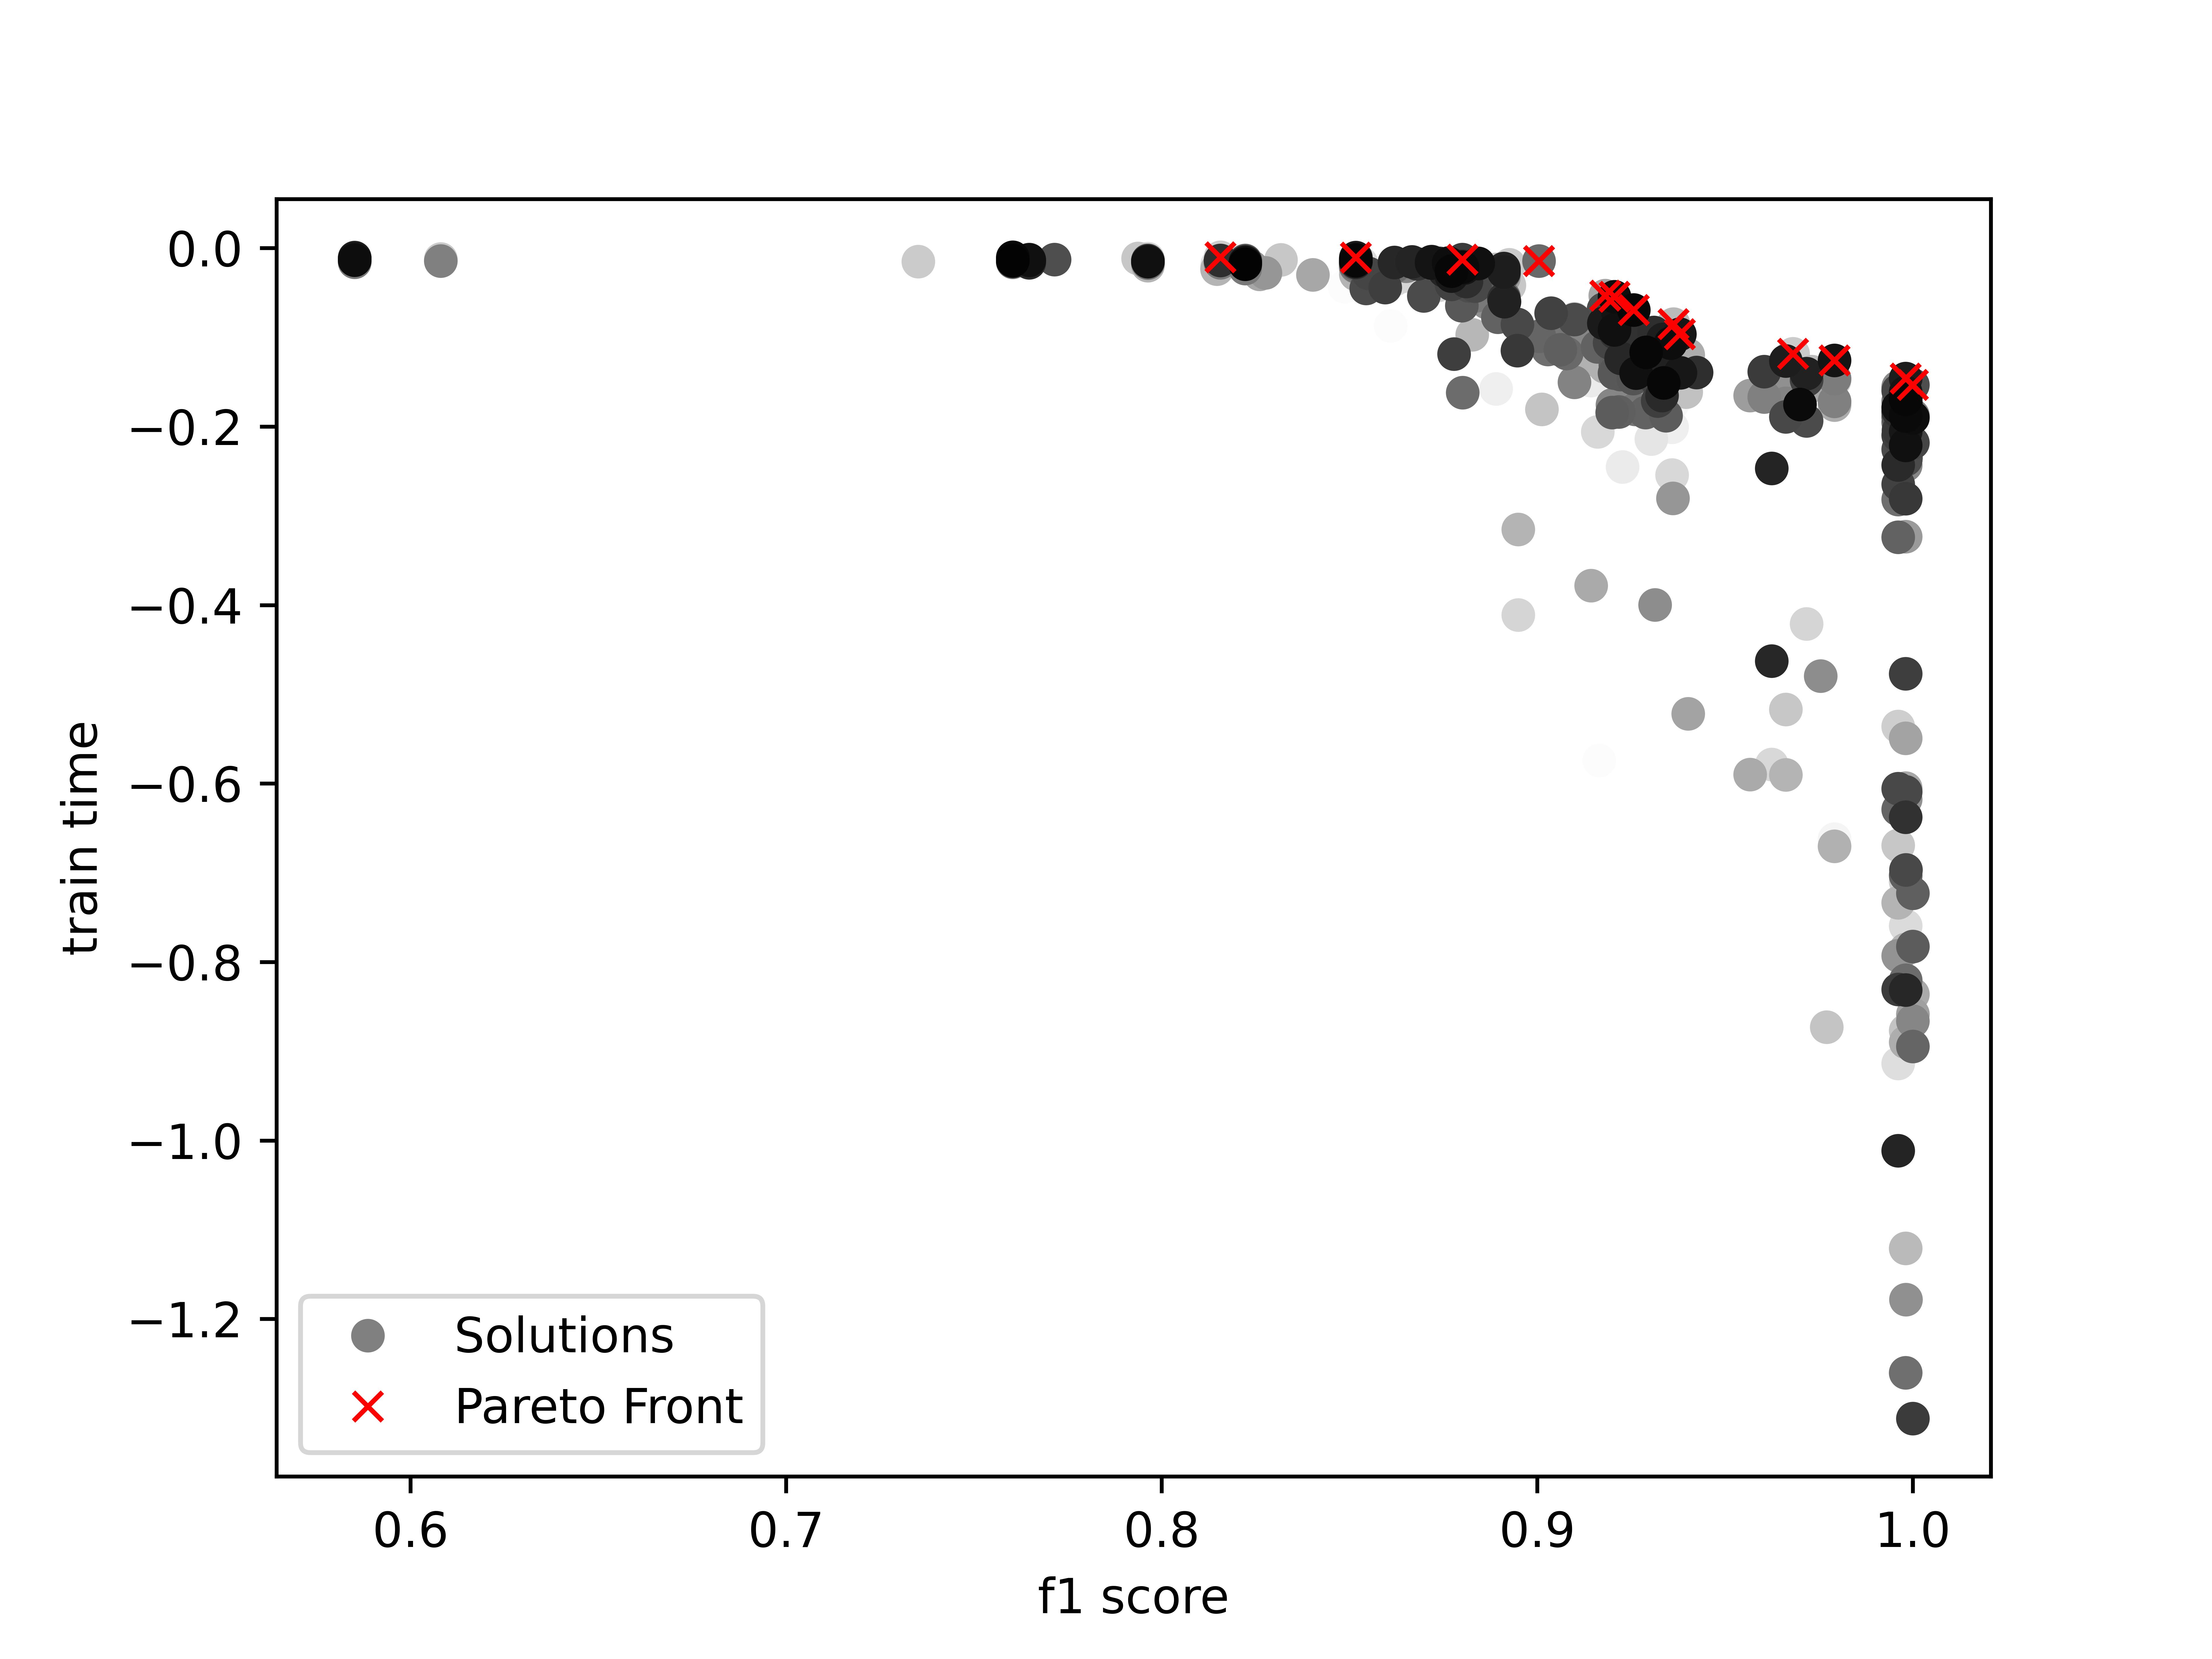
\includegraphics[scale=0.65]{Pictures/cars_fscore_vs_time.jpg}
    \caption{Cars: F-score contra Tiempo de Entrenamiento}
    \label{impl:fig:cars:fscore_vs_time}
\end{figure}


\subsubsection{Precisi\'on contra Recobrado}
Durante esta prueba ocurre un hecho interesante, ni precisi\'on ni recobrado entr\'an en conflicto y por tanto no es necesario hacer concesiones entre una o la otra durante la optimizaci\'on. Se puede observar observa en la figura \ref{impl:fig:cars:precision_vs_recall} que el frente de Pareto esta consituido por un s\'olo punto donde se maximizan precision y recobrado. Tambi\'en se nota como las soluciones van mejorando con el transcurso de las iteraciones.
Adem\'as AutoGOAL encontr\'o 30 soluciones distintas con respecto a algoritmos e hyperpar\'ametros que logran este rendimiento y podri\'ia ser interesante para el investigador analizar las diferencias entre estas.

\begin{figure}[ht]
    \centering
    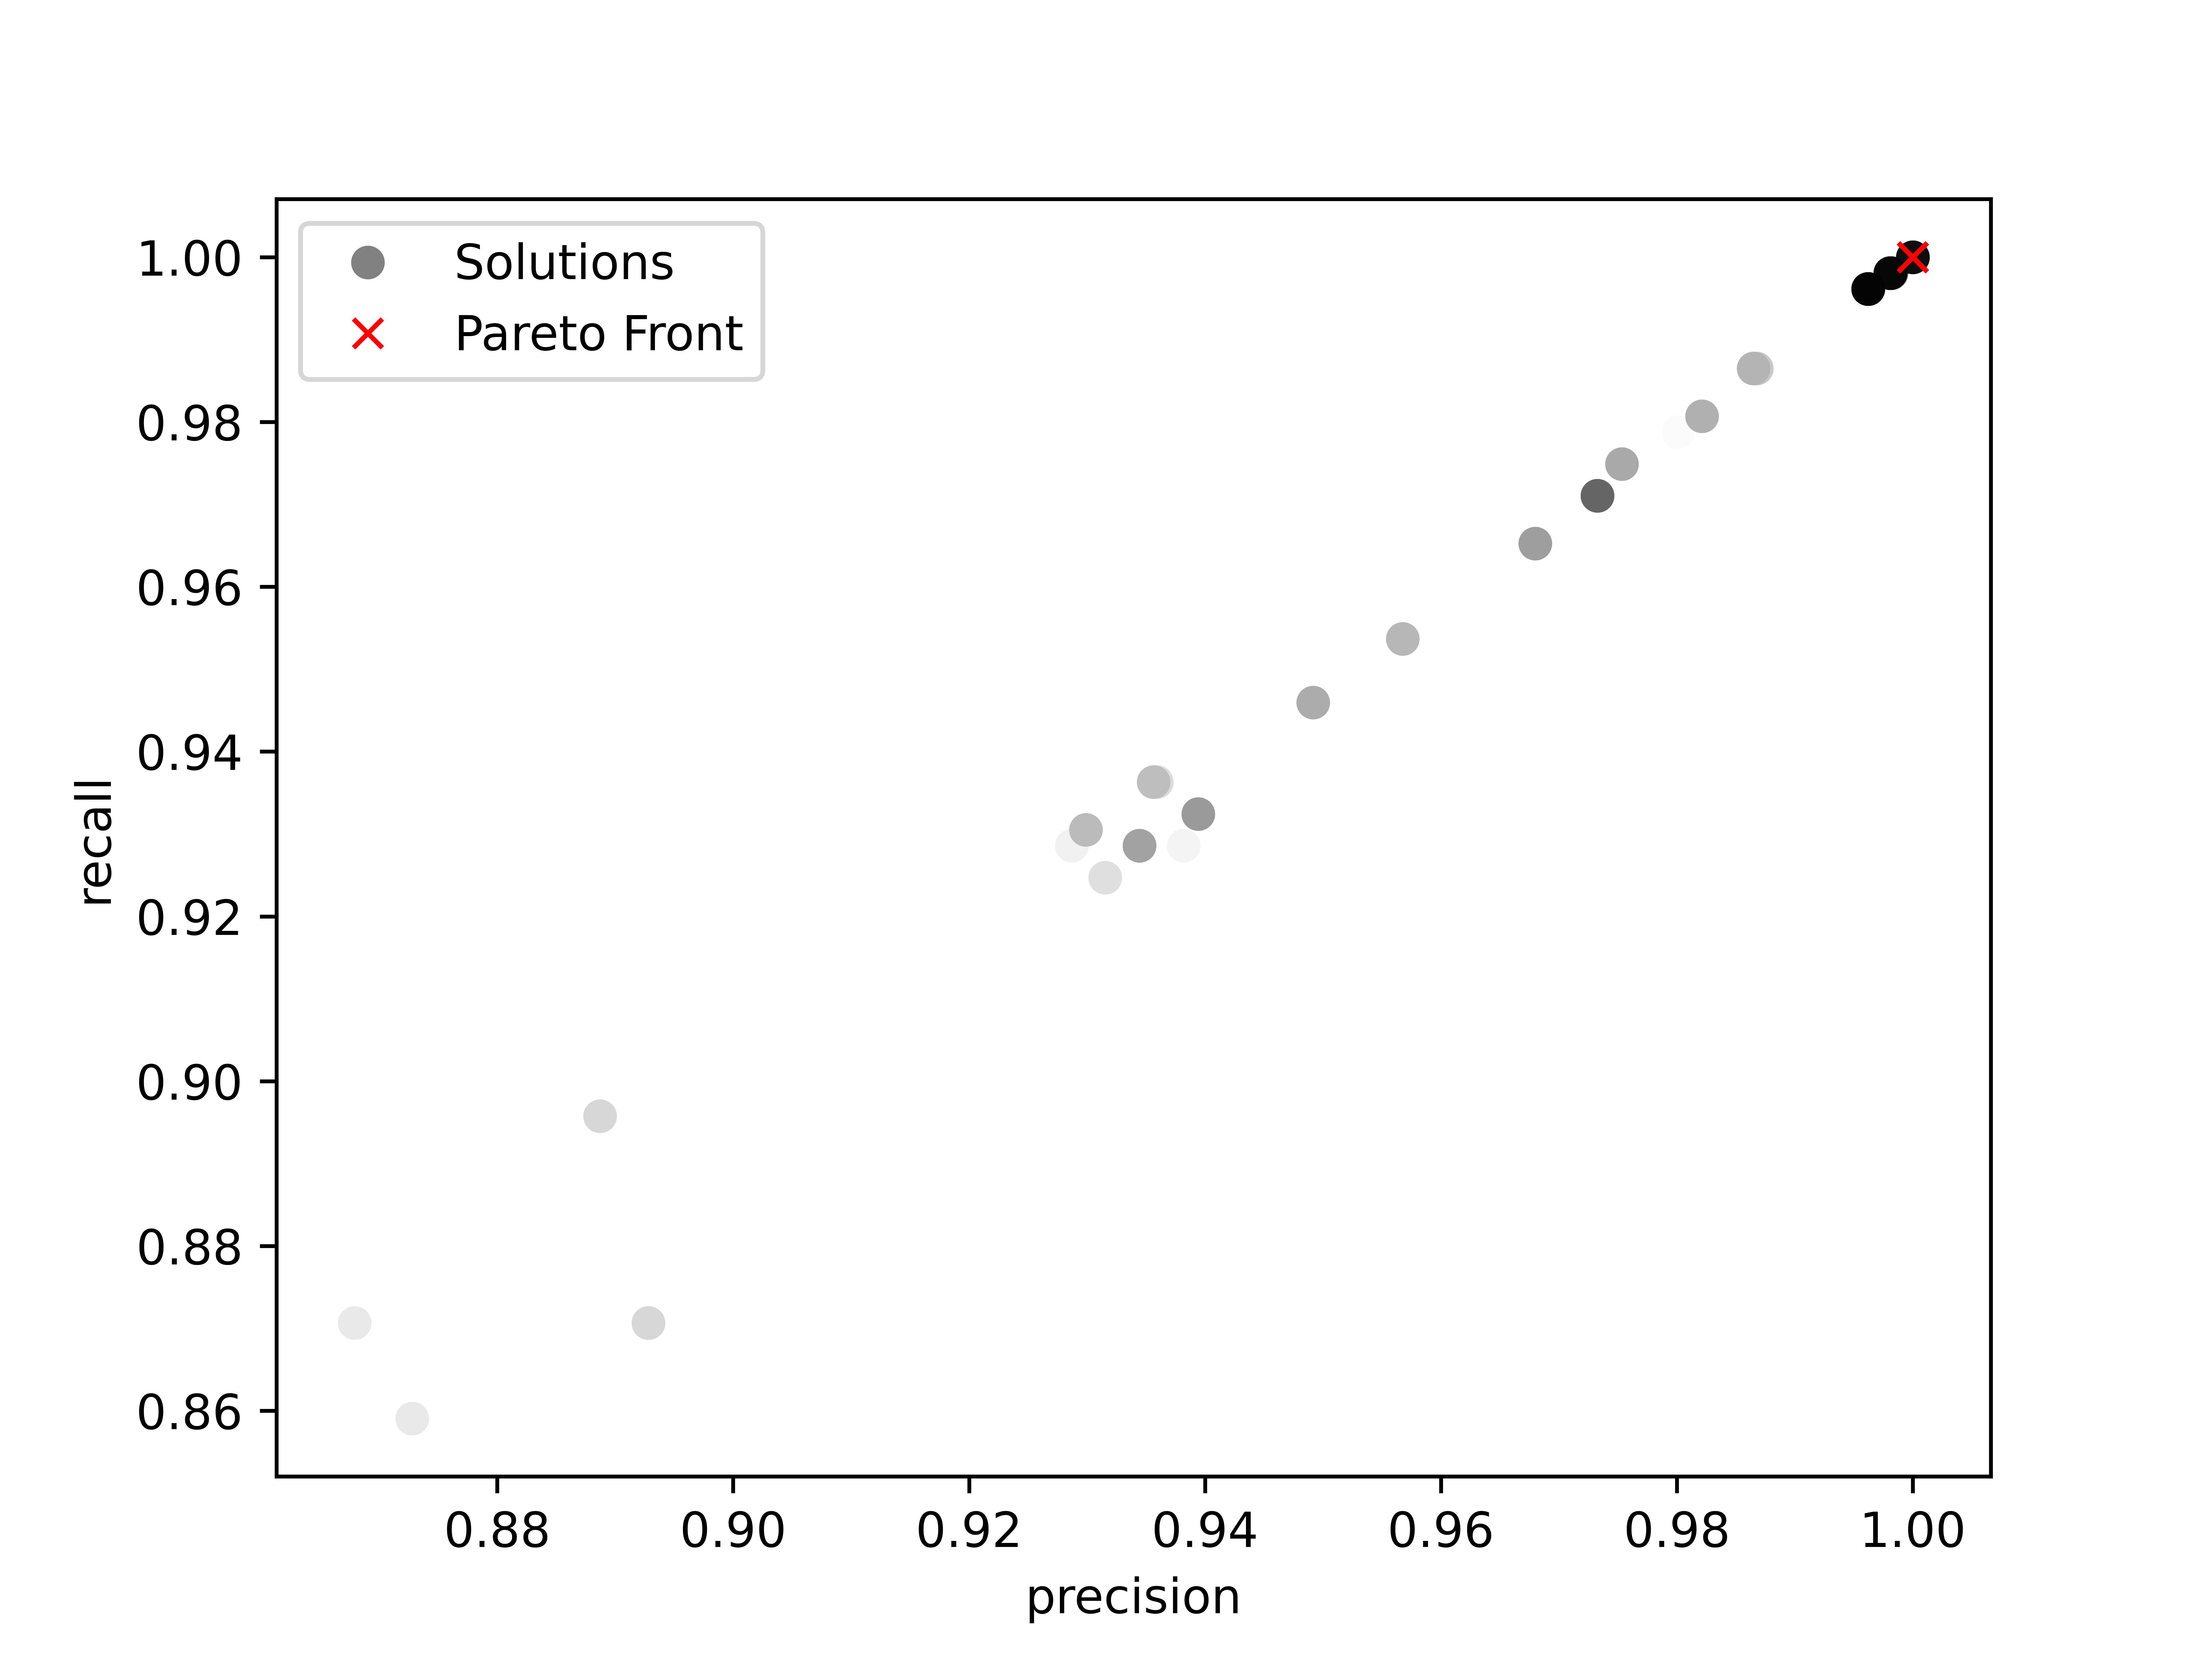
\includegraphics[scale=0.65]{Pictures/cars_precision_vs_recall.jpg}
    \caption{Cars: Precisi\'on contra Recobrado}
    \label{impl:fig:cars:precision_vs_recall}
\end{figure}

\subsection{HAHA}
Se utilzo una poblaci\'on total de 40 individuos, 8 horas de tiempo m\'aximo y 10 segundos por  evaluaci\'on. 
HAHA es un problema de clasificaci\'on binario y por las m\'etricas \textit{f-score}, precisi\'on y recobrado son las implementadas en Scikit utilizando promedio binario 

\subsubsection{F-Score contra Tiempo de Entrenamiento}

En esta prueba el frente como se observa en la figura \ref{impl:fig:haha:fscore_vs_time} posee una forma aparentemente similar a \ref{impl:fig:cars:fscore_vs_time}. 

Los pipelines de AutoGOAL en esta ocasi\'on est\'an conformados por dos algoritmos principales. Los que contienen poca precisi\'on pero son general m\'as rapidos est\'an conformados por HasingVectorizer y NearestCentroid y  lo que varia entre ellas son los hiperparametros.

Los que tienen mayor precision a costo de un poco de tiempo est\'an compuestos por count vectorizer  y regresores log\'isticos.

Adem\'as en la esquina superior izquierda se ve como AutoGOAL busca un punto que tiene f-score 0, una soluci\'on completamente in\'util y donde se desperdicia tiempo de c\'omputo; no obstatne, el sistema es agn\'ostico a esto. Una posible mitigaci\'on contra estos casos ser\'ia permitir a el usuario establecer restricciones sobre los valores de ciertas m\'etricas. Adem\'as en el caso de muchas m\'etricas puede ser \'util  tener un lenguage suficientemente expresivo que permita describir secciones del espacio que no interesan. En este caso, se restringiria a \textit{f-score} $\> 0$.

\begin{figure}[ht]
    \centering
    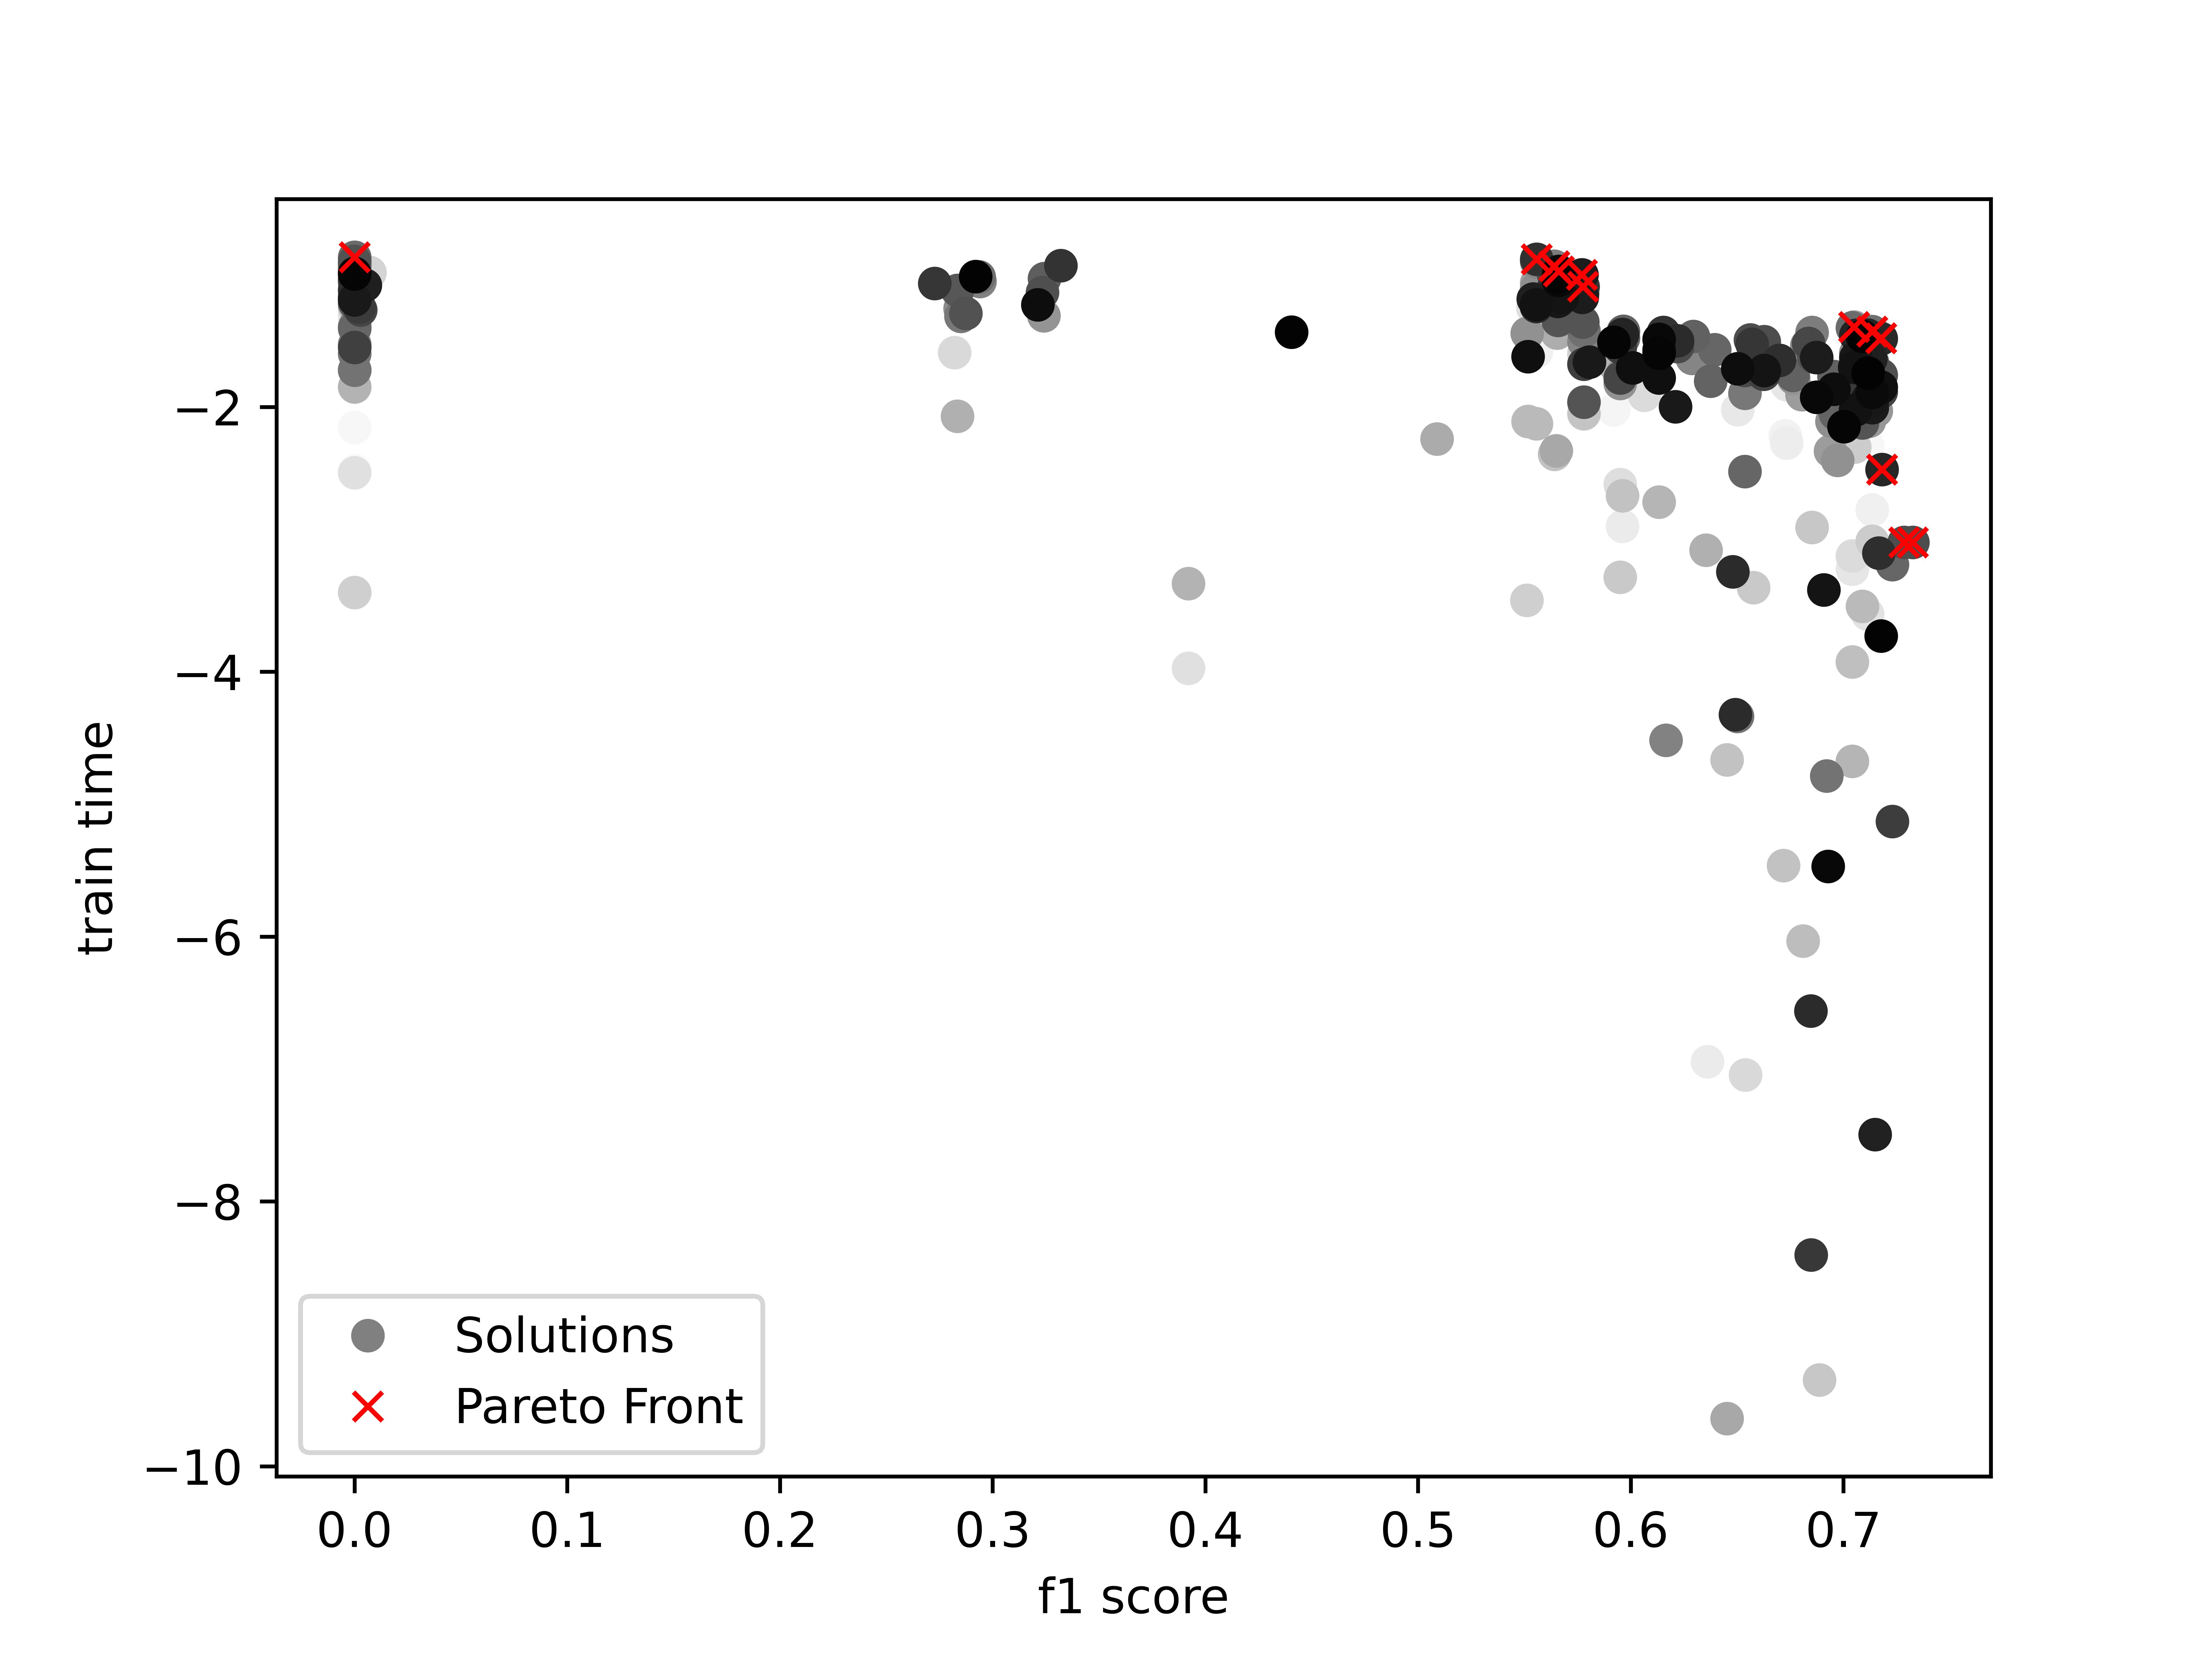
\includegraphics[scale=0.65]{Pictures/haha_fscore_vs_time.jpg}
    \caption{HAHA: F-score contra Tiempo de Entrenamiento (10 segundos m\'ax)}
    \label{impl:fig:haha:fscore_vs_time}
\end{figure}

Otra de las cosas a notar es que hay algoritmos que toman 10 segundos para ejecutarse, lo que sugiere que el espacio se restringe a 10 segundos respecto a la m\'etrica de tiempo de entrenamiento. Se realiza una segunda prueba extendiendo esta restricci\'on hasta 3 minutos con el fin de verificar si aumentando el esapcio de b\'usqueda se puede obtener una representaci\'on distinta del frente de Pareto. En este caso la estructura extra\~na del frente se mantiene, no obstante aparece una nueva soluc\'on que diferente al resto donde se obtiene un \textit{f-score} cercano a 0.8 pero con un costo de entrenamiento de 30 segundos.

\begin{figure}[ht]
    \centering
    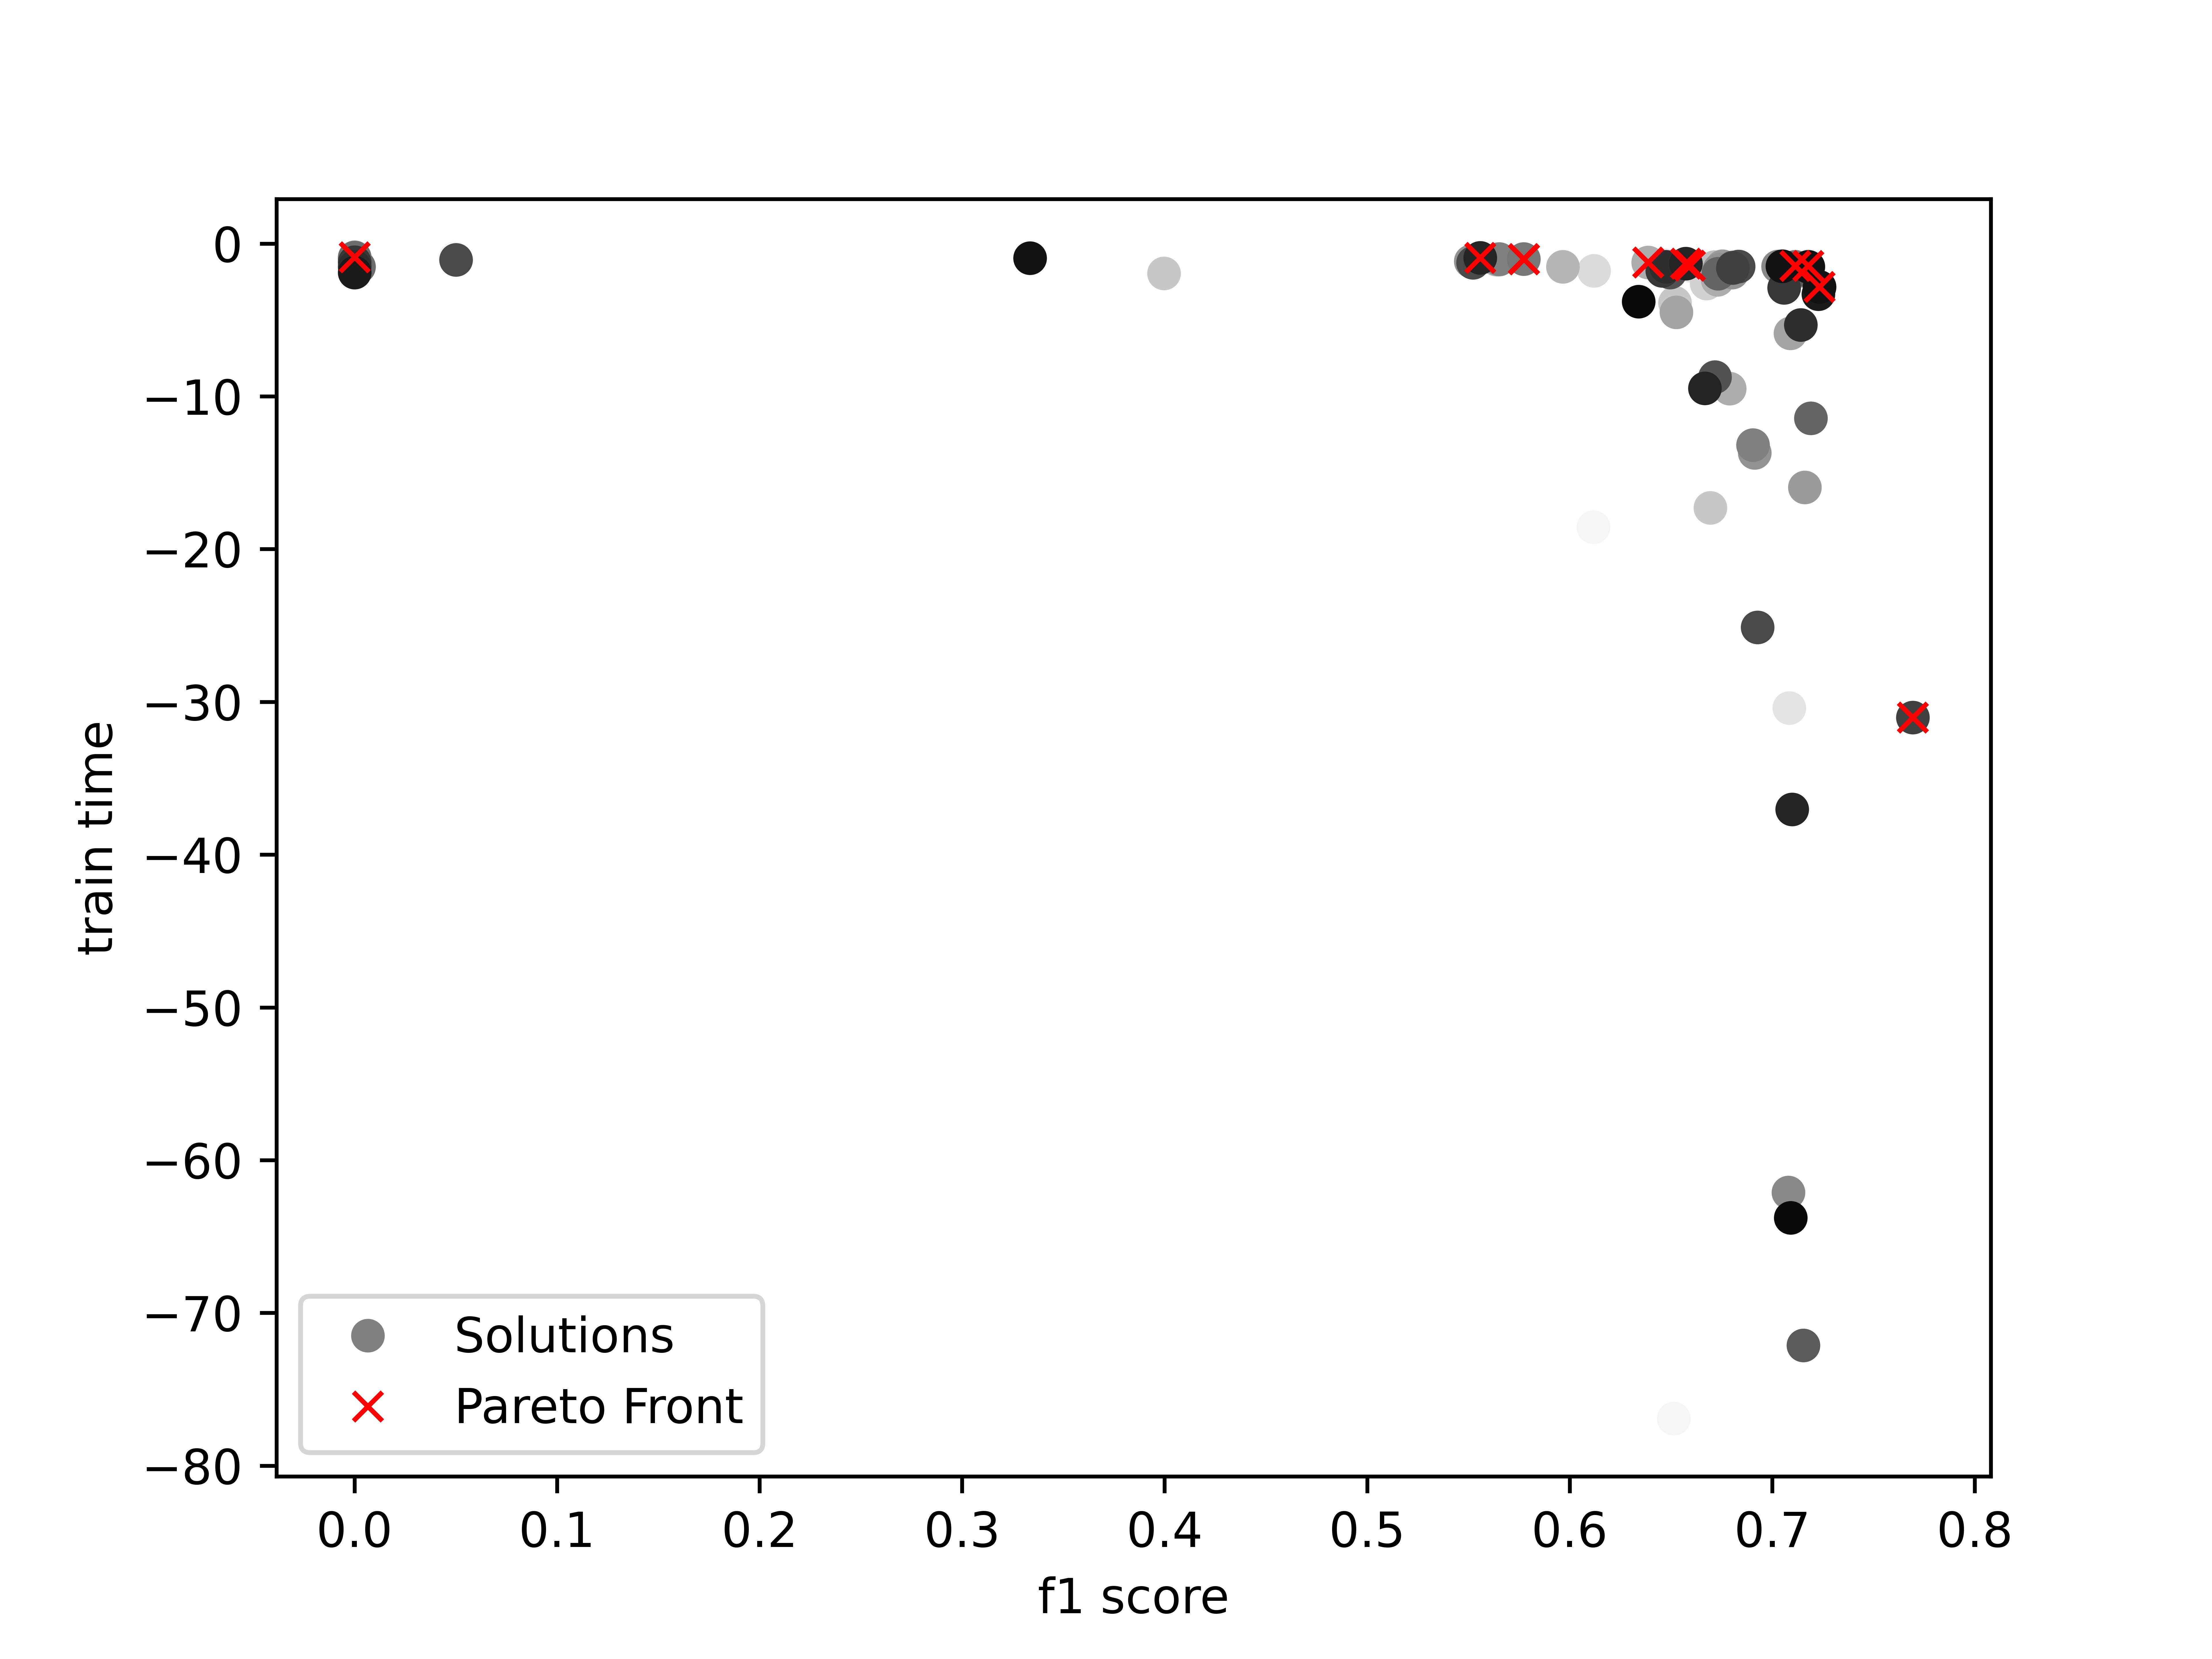
\includegraphics[scale=0.65]{Pictures/haha_fscore_vs_time_3min.jpg}
    \caption{HAHA: F-score contra Tiempo de Entrenamiento (3 minutos m\'ax)}
    \label{impl:fig:haha:fscore_vs_time_3min}
\end{figure}

\subsubsection{Precisi\'on contra Recobrado}
Contrario a lo que muestra la evaluaci\'on de Cars con respecto a precision y recobrado, durante esta prueba no es posible encontrar un flujo que maximice ambas m\'etricas y es necesario hacer concesiones entre una y la otra. El frente como se observa en la figura \ref{impl:fig:haha:precision_vs_recall} tiene una forma c\'onvexa, consecuencia del conflicto que se crea al optimizar para varias m\'etricas en este conjunto de datos.

\begin{figure}[ht]
    \centering
    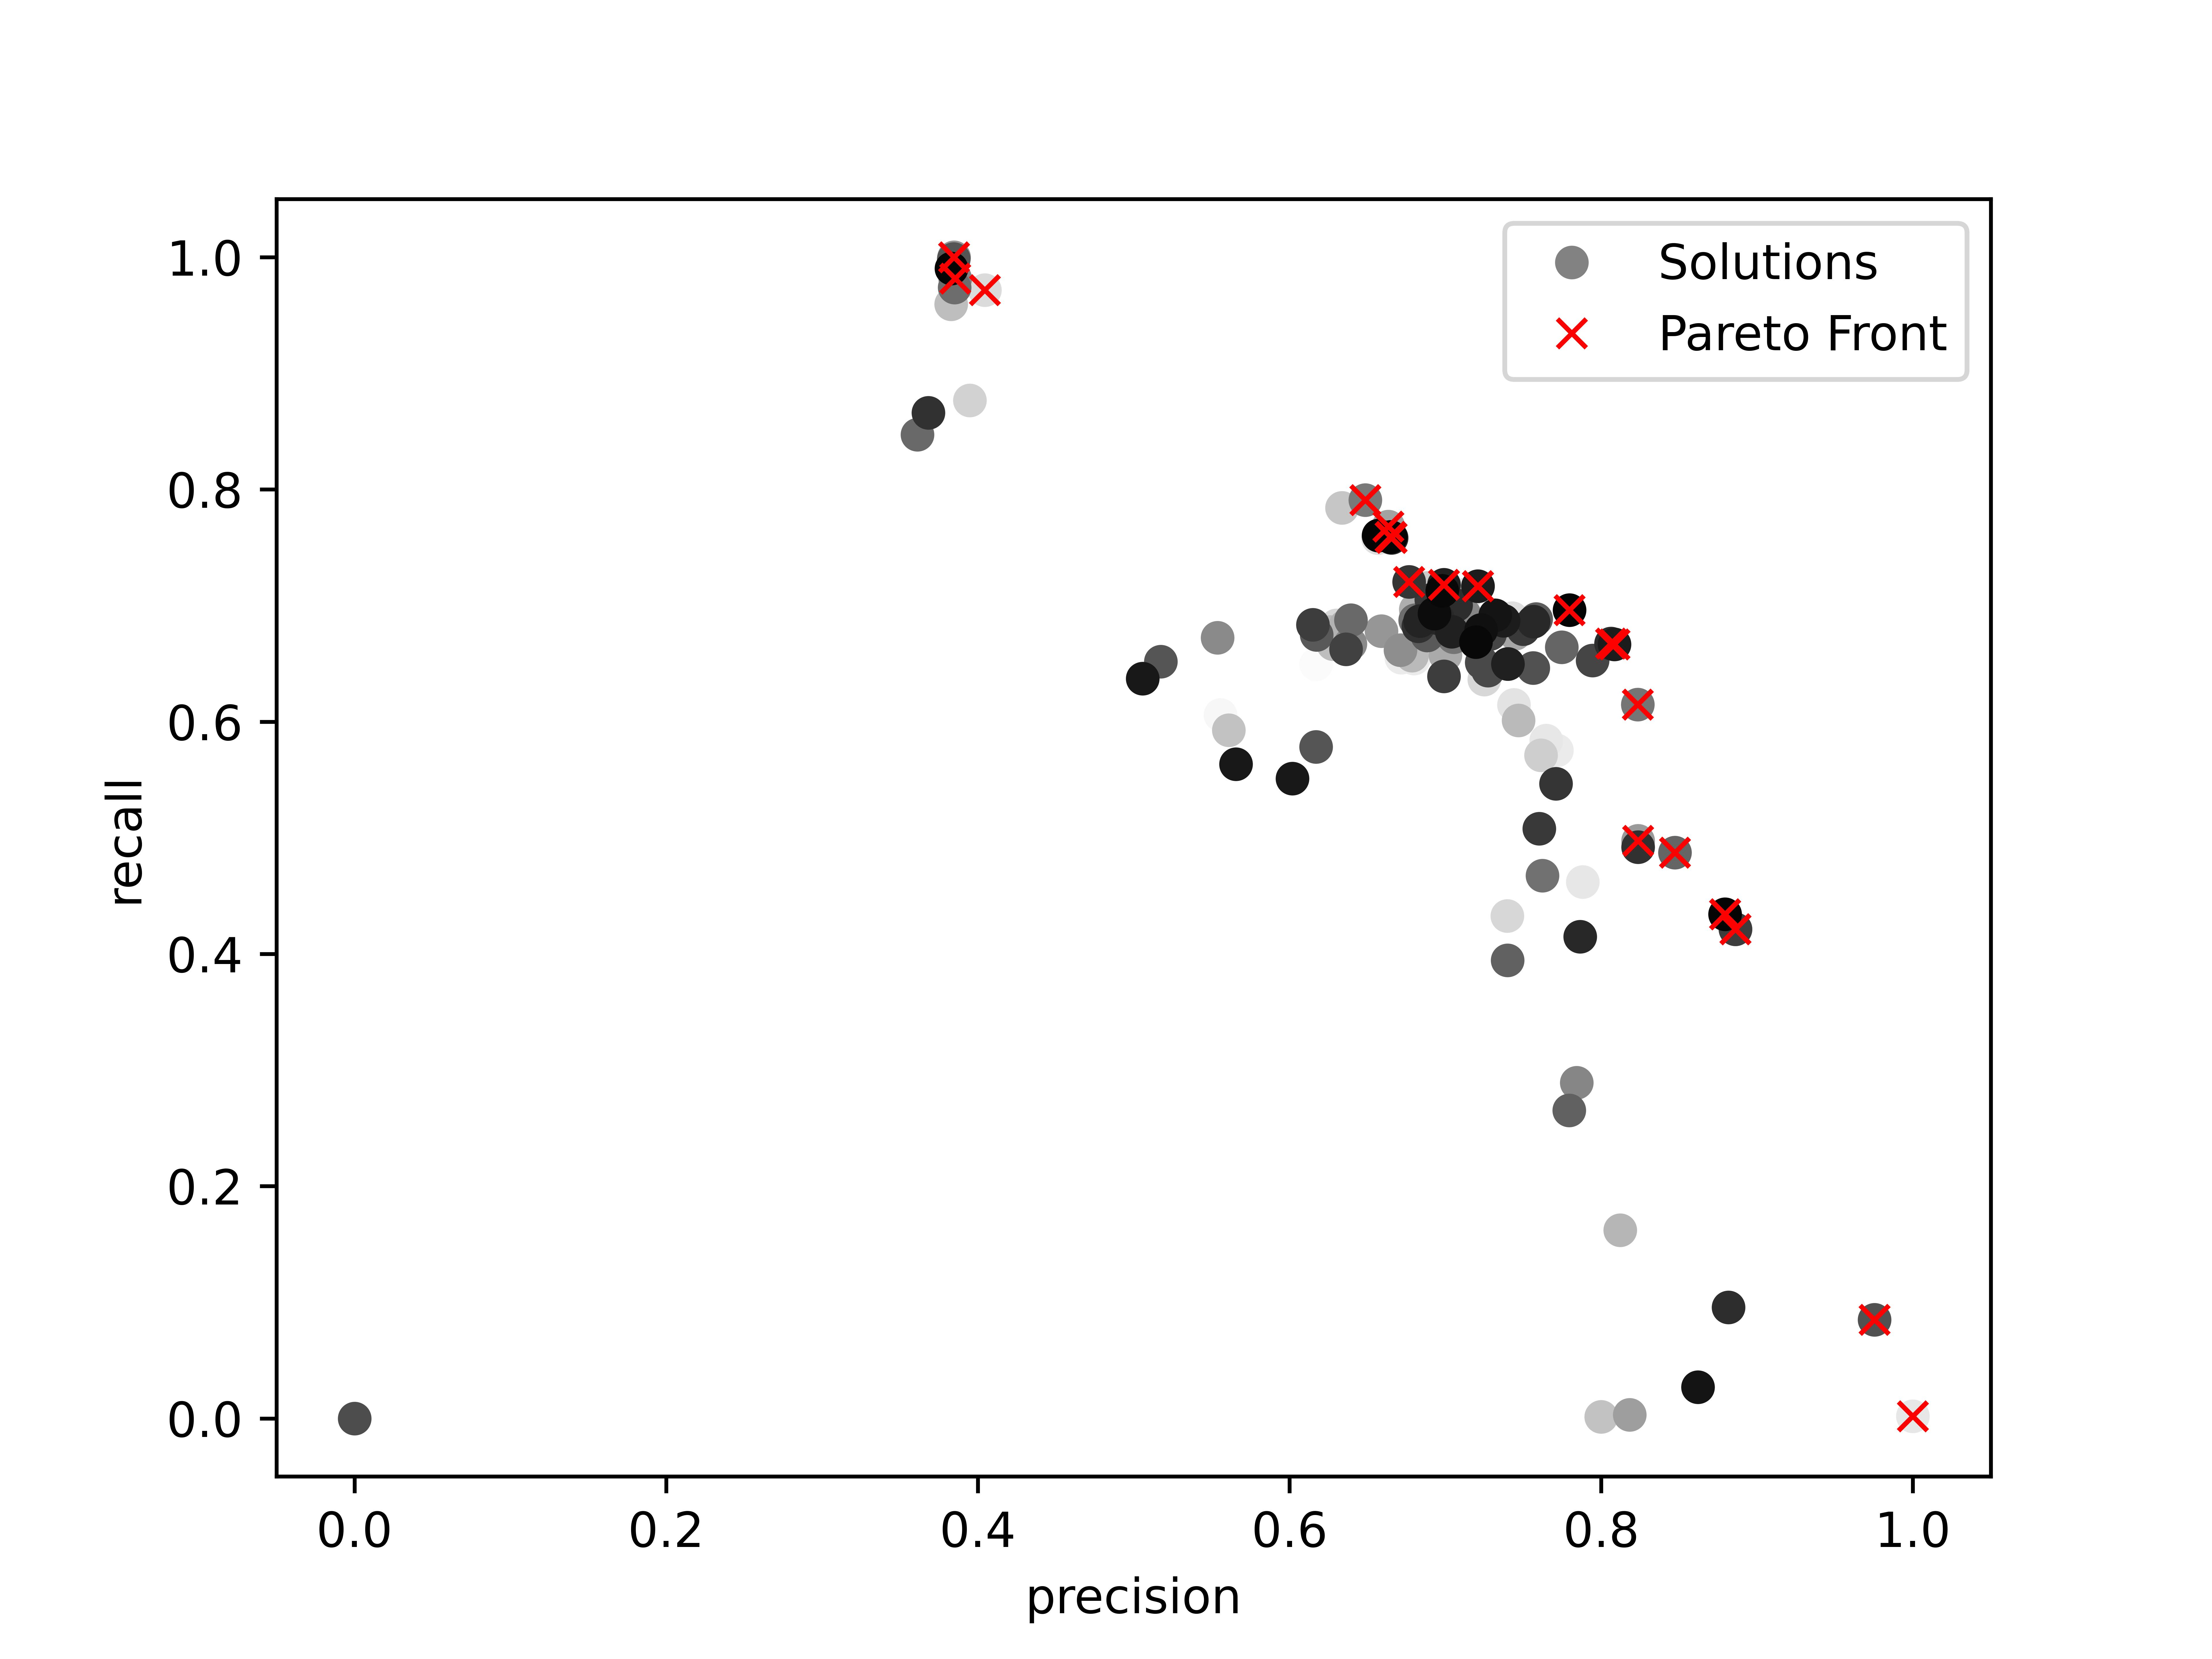
\includegraphics[scale=0.65]{Pictures/haha_precision_vs_recall.jpg}
    \caption{HAHA: Precisi\'on contra Recobrado (10 segundos m\'ax)}
    \label{impl:fig:haha:precision_vs_recall}
\end{figure}

Cuando se optimza con tiempo m\'aximo de tres minutos no se muestra ning\'un cambio notable con respecto a la anterior prueba. 

\begin{figure}[ht]
    \centering
    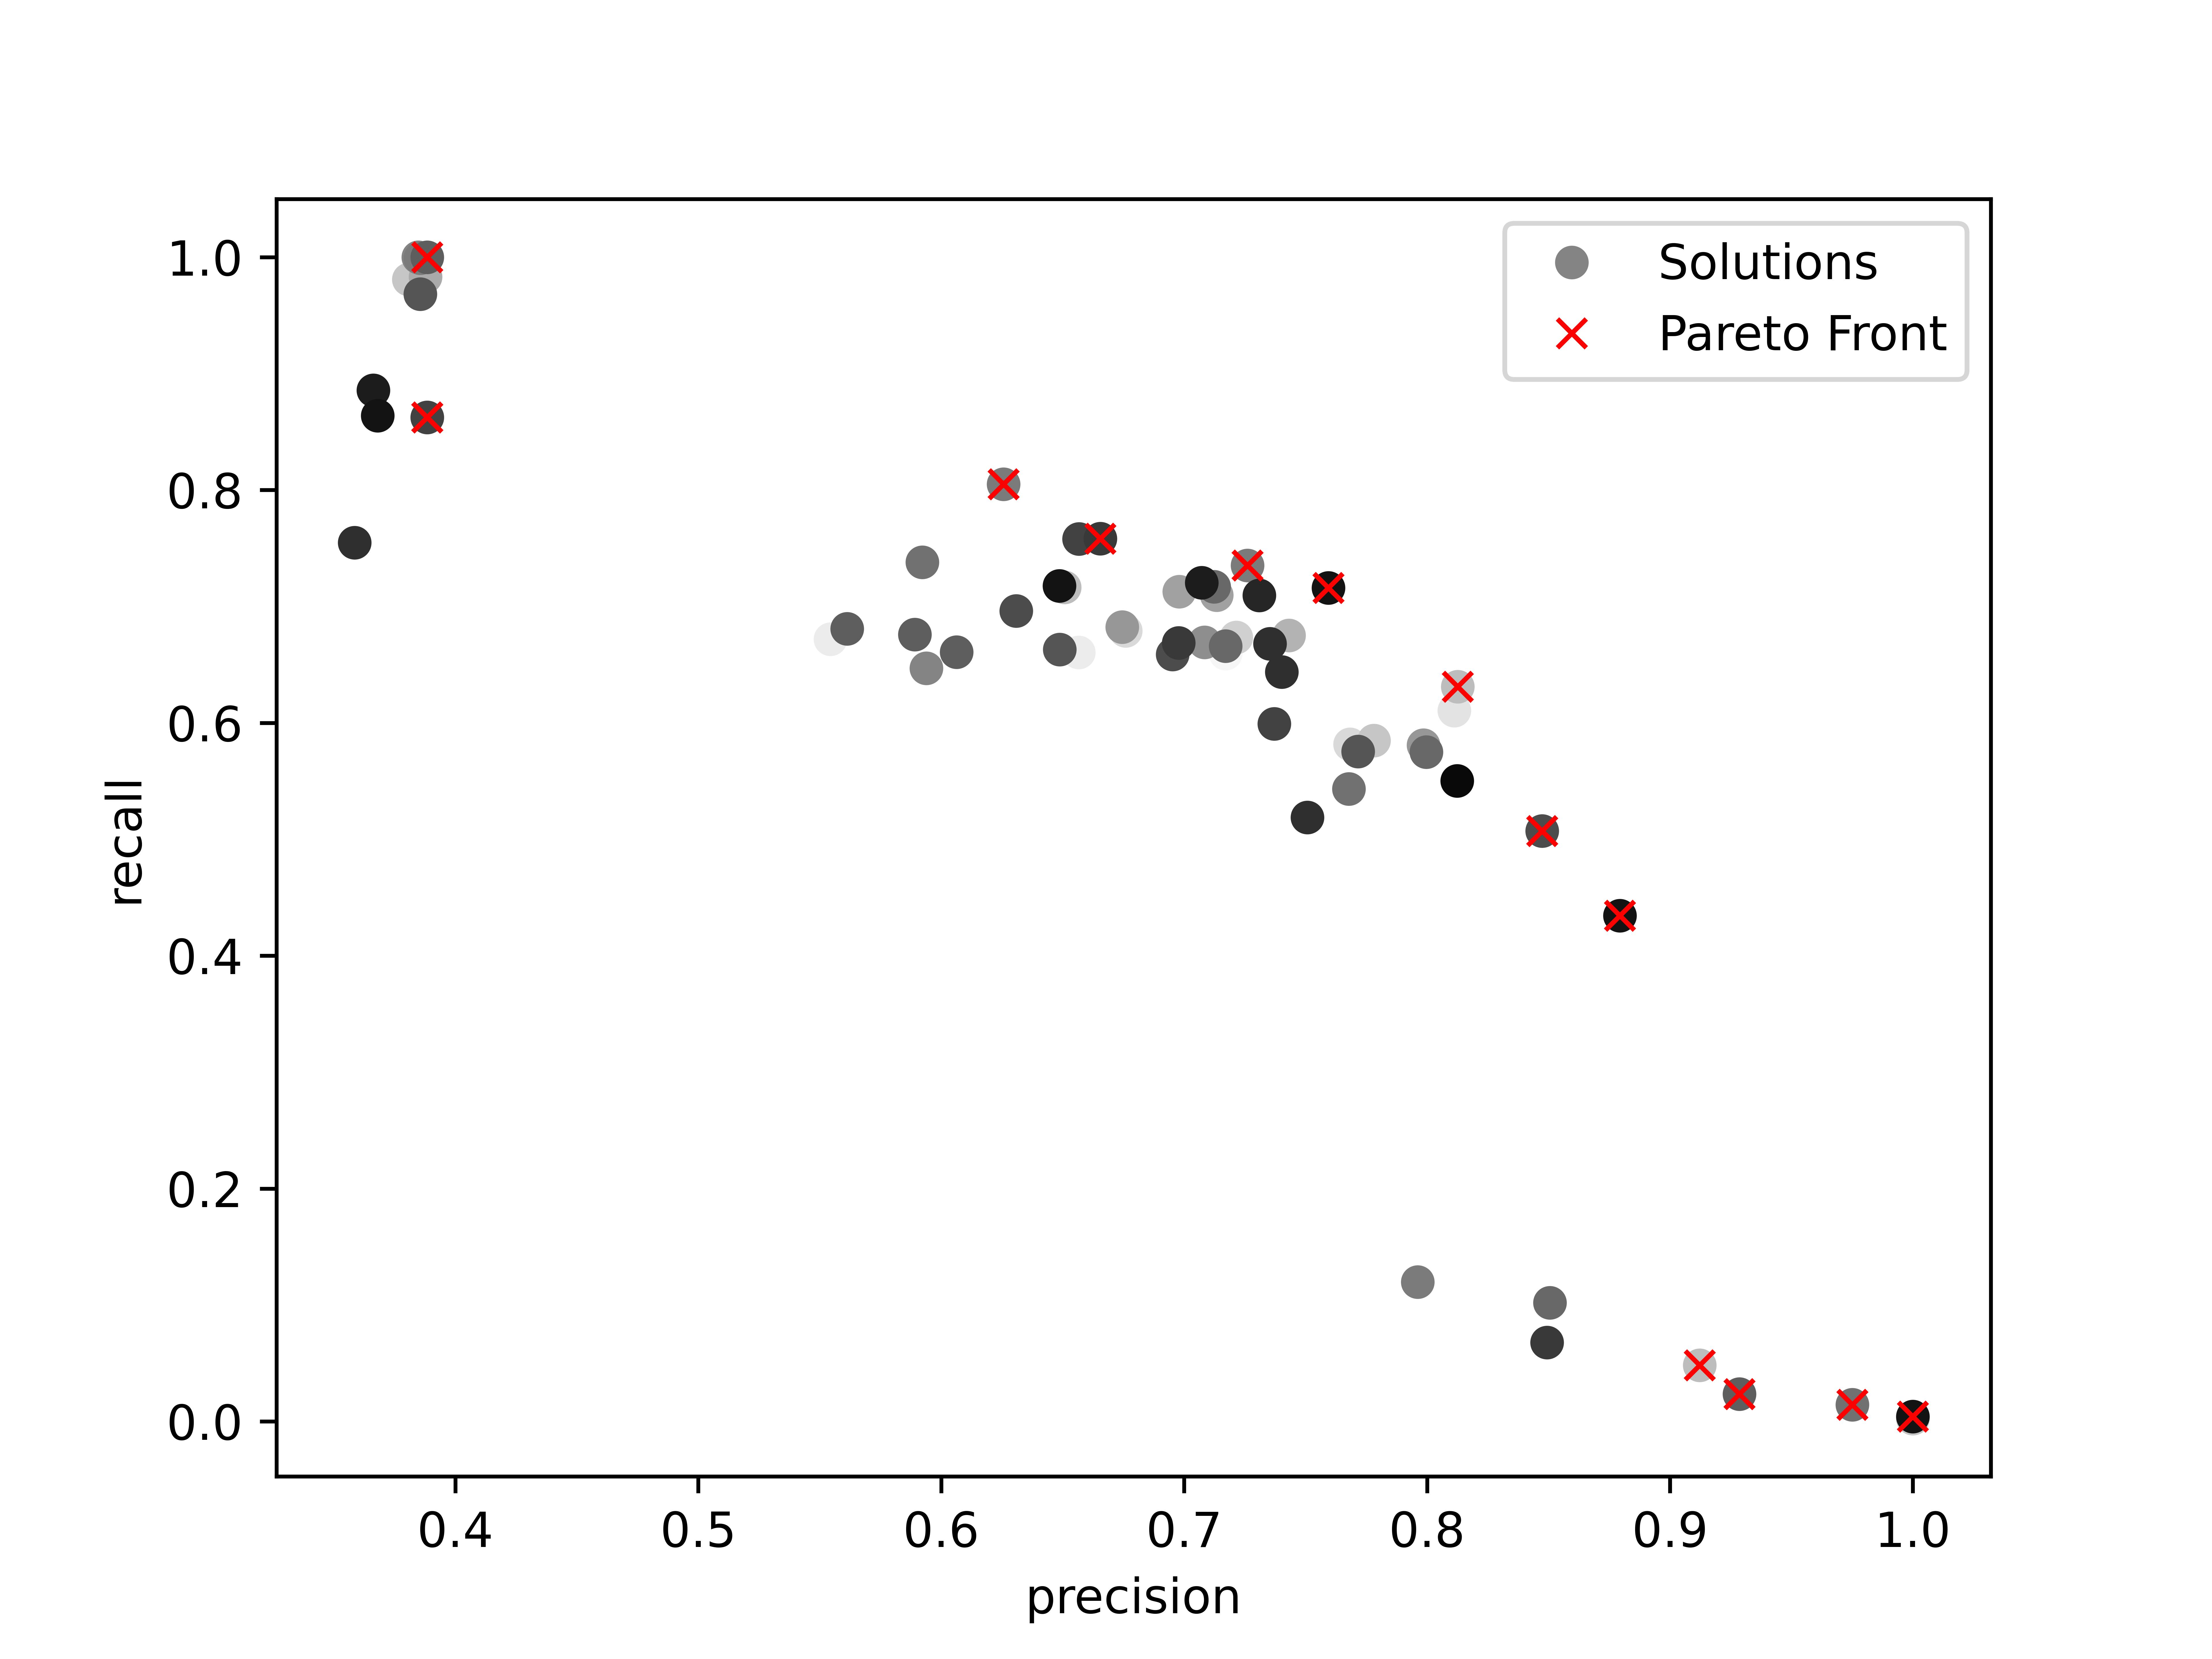
\includegraphics[scale=0.65]{Pictures/haha_precision_vs_recall_3min.jpg}
    \caption{HAHA: Precisi\'on contra Recobrado (3 minutos m\'ax)}
    \label{impl:fig:haha:precision_vs_recall_3min}
\end{figure}

\subsection{MEDDOCAN}

Se utilzo una poblacion total de 50 individuos, 10 horas de tiempo m\'aximo y 10 mintuos por  evaluaci\'on. 

Este corpus representa el conjunto de datos m\'as grande de los tres y por ende fue necesario aumentar el tiempo de evaluaci\'on por flujo a 10 minutos, con el fin de encontrar soluciones validas, estas tomando tiempes de entre 2 y 6 minutos. Las pruebas se corrieron con una poblaci\'on total de 50 individuos, 10 horas de tiempo m\'aximo y 10 minutos por evaluaci\'on. 
Las implementaciones de \textit{f-score}, precisi\'on y recobrado son las implementaciones del m\'odulo de Python \textit{meddocan}.
El entrenamiento en esta prueba resultaron ser m\'as lentos y no fue posible realizar muchas iteraciones por lo que no es posible apreciar completamente los frentes.
% Aqu\'i el tiempo m\'aximo es mucho mayor pues es un corpus es mucho m\'as grande que los anteriores que para encontrar al menos un pipeline v\'alido require alrededor de 7 u 8 minutos. Lo suficiente para lograr 3 o 4 generaciones de un total de 100.


\subsubsection{F-Score contra Tiempo de Entrenamiento}

En esta prueba se ve un comportamiento similar a las anteriores como puede observar en la figura  \ref{impl:fig:MEDDOCAN:fscore_vs_train_time} quizas un poco m\'as acentuado debido al incremento en los tiempos de entrenamiento.

\begin{figure}[ht]
    \centering
    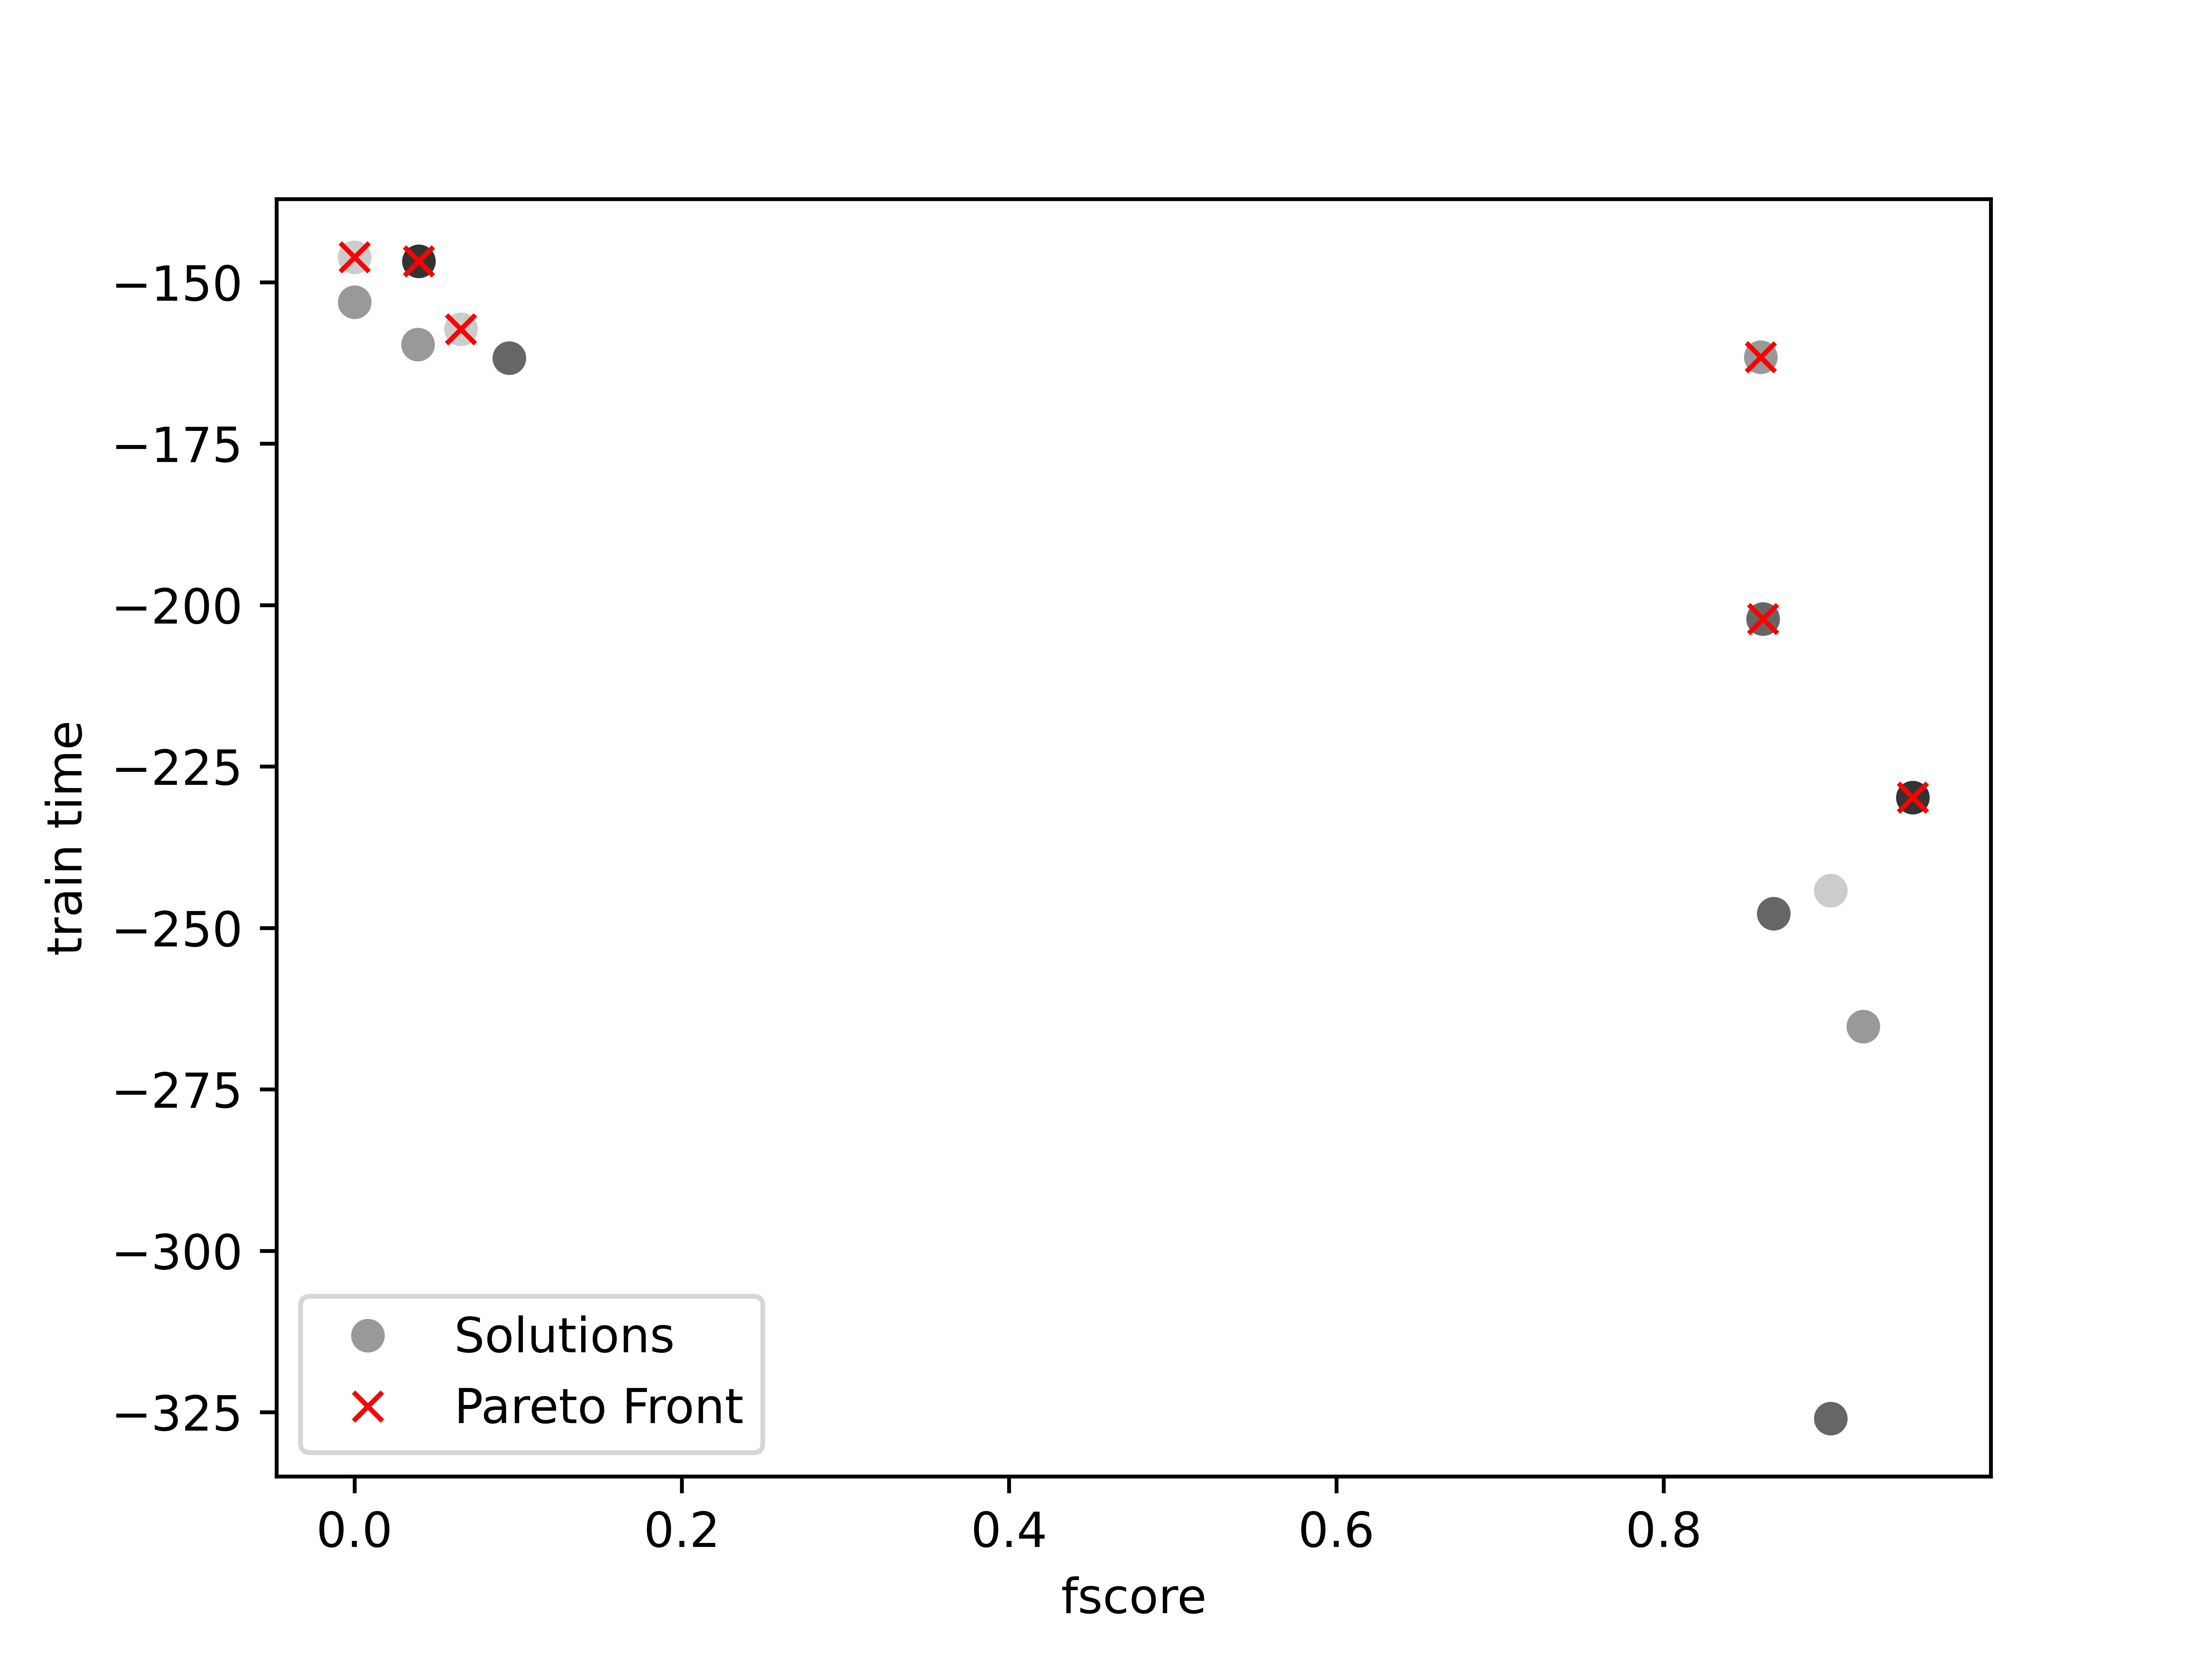
\includegraphics[scale=0.65]{Pictures/meddocan_fscore_vs_train.jpg}
    \caption{MEDDOCAN: F-Score contra Tiempo de Entrenamiento}
    \label{impl:fig:MEDDOCAN:fscore_vs_train_time}
\end{figure}


\subsubsection{Precisi\'on contra Recobrado}

En esta figura \ref{impl:fig:MEDDOCAN:precision_vs_recall} debido a la poca cantiad de iteraciones se obtiene una representaci\'on muy probre del frente de Pareo. No queda claro si estamos frente a un caso parecido al de \ref{impl:fig:cars:precision_vs_recall} donde las m\'etricas no entran en conflicto y es posible optimizar para ambas, o mas parecido al caso en \ref{impl:fig:HAHA:precision_vs_recall} dodne es obligatorio realizar trade offs.

\begin{figure}[ht]
    \centering
    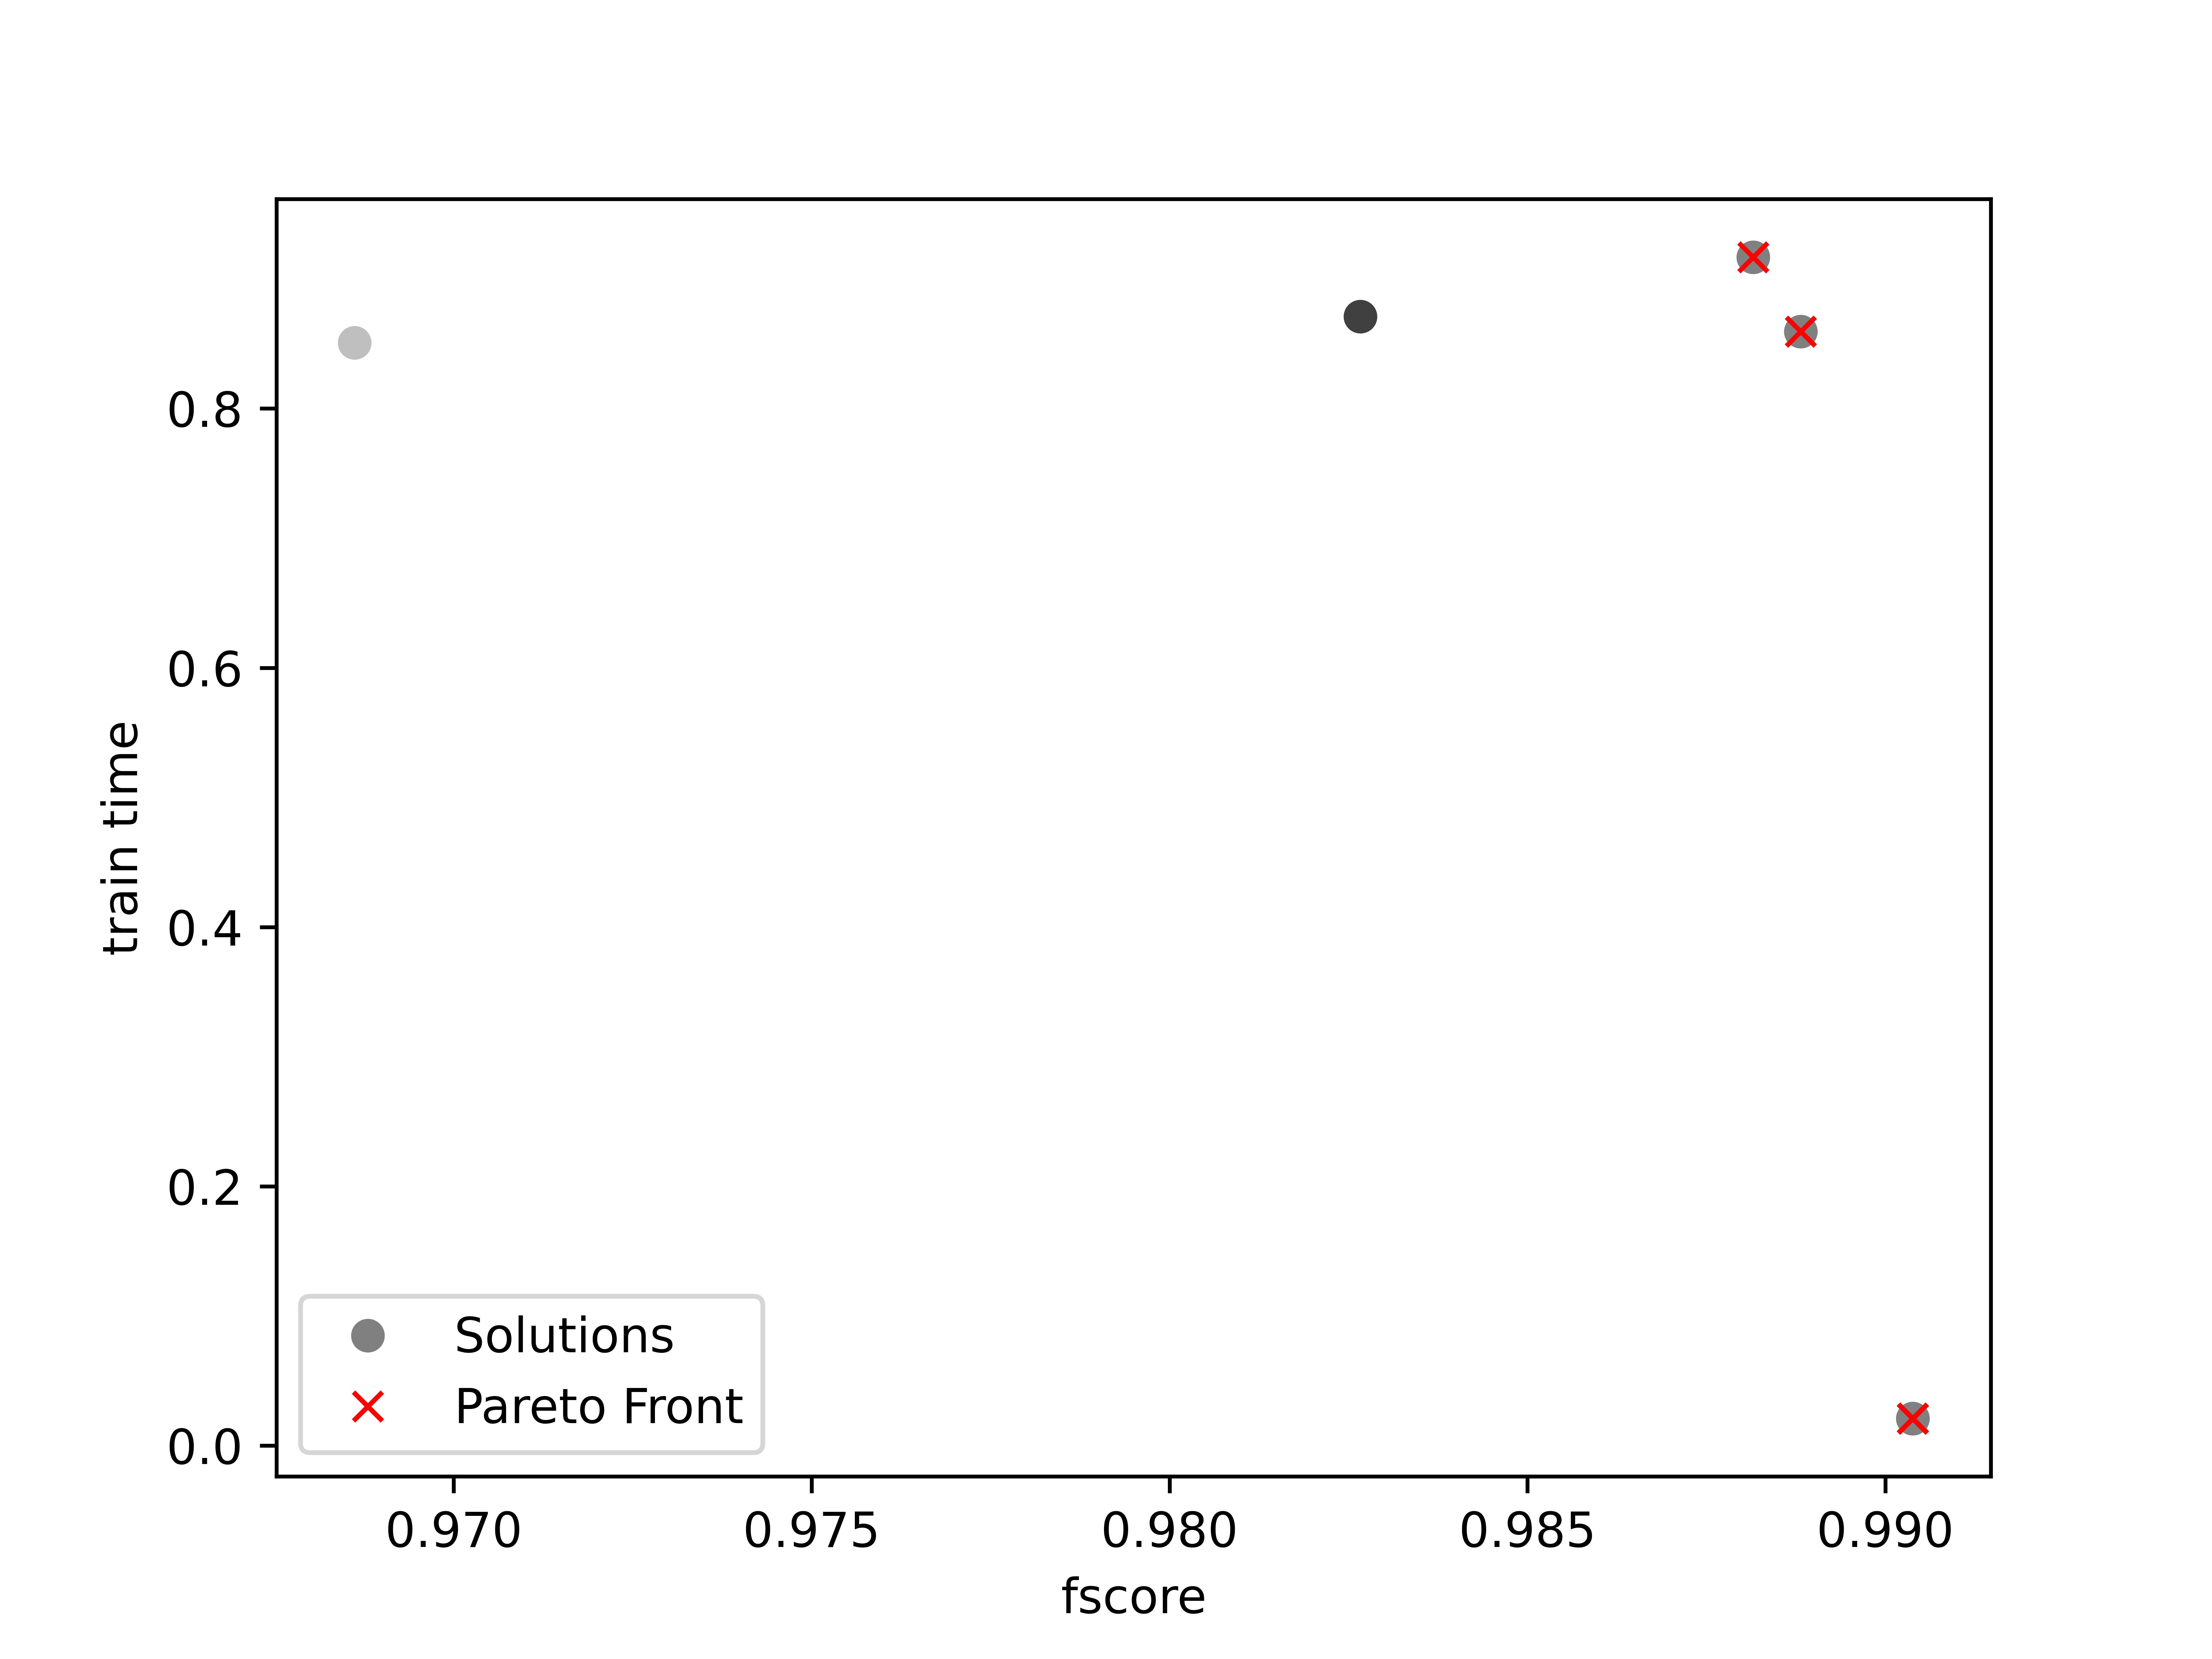
\includegraphics[scale=0.65]{Pictures/meddocan_precision_vs_recall.jpg}
    \caption{MEDDOCAN: Precisi\'on contra Recobrado}
    \label{impl:fig:MEDDOCAN:precision_vs_recall}
\end{figure}
